\documentclass[12pt]{beamer}
\usepackage{../Estilos/BeamerFC}
\usepackage{../Estilos/ColoresLatex}
\usepackage{courier}
\usepackage{listingsutf8}
\usepackage{listings}
\usepackage{xcolor}
\usepackage{textcomp}
\usepackage{color}
\definecolor{deepblue}{rgb}{0,0,0.5}
\definecolor{brown}{rgb}{0.59, 0.29, 0.0}
\definecolor{OliveGreen}{rgb}{0,0.25,0}
% \usepackage{minted}

\DeclareCaptionFont{white}{\color{white}}
\DeclareCaptionFormat{listing}{\colorbox{gray}{\parbox{0.98\textwidth}{#1#2#3}}}
\captionsetup[lstlisting]{format=listing,labelfont=white,textfont=white}
\renewcommand{\lstlistingname}{Código}


\definecolor{Code}{rgb}{0,0,0}
\definecolor{Keywords}{rgb}{255,0,0}
\definecolor{Strings}{rgb}{255,0,255}
\definecolor{Comments}{rgb}{0,0,255}
\definecolor{Numbers}{rgb}{255,128,0}

\makeatletter

\newif\iffirstchar\firstchartrue
\newif\ifstartedbyadigit
\newif\ifprecededbyequalsign

\newcommand\processletter
{%
  \ifnum\lst@mode=\lst@Pmode%
    \iffirstchar%
        \global\startedbyadigitfalse%
      \fi
      \global\firstcharfalse%
    \fi
}

\newcommand\processdigit
{%
  \ifnum\lst@mode=\lst@Pmode%
      \iffirstchar%
        \global\startedbyadigittrue%
      \fi
      \global\firstcharfalse%
  \fi
}

\lst@AddToHook{OutputOther}%
{%
  \lst@IfLastOtherOneOf{=}
    {\global\precededbyequalsigntrue}
    {}%
}

\lst@AddToHook{Output}%
{%
  \ifprecededbyequalsign%
      \ifstartedbyadigit%
        \def\lst@thestyle{\color{orange}}%
      \fi
    \fi
  \global\firstchartrue%
  \global\startedbyadigitfalse%
  \global\precededbyequalsignfalse%
}

\lstset{ 
language=Python,                % choose the language of the code
basicstyle=\footnotesize\ttfamily,       % the size of the fonts that are used for the code
numbers=left,                   % where to put the line-numbers
numberstyle=\scriptsize,      % the size of the fonts that are used for the line-numbers
stepnumber=1,                   % the step between two line-numbers. If it is 1 each line will be numbered
numbersep=5pt,                  % how far the line-numbers are from the code
backgroundcolor=\color{white},  % choose the background color. You must add \usepackage{color}
showspaces=false,               % show spaces adding particular underscores
showstringspaces=false,         % underline spaces within strings
showtabs=false,                 % show tabs within strings adding particular underscores
frame=single,   		% adds a frame around the code
tabsize=2,  		% sets default tabsize to 2 spaces
captionpos=t,   		% sets the caption-position to bottom
breaklines=true,    	% sets automatic line breaking
breakatwhitespace=false,    % sets if automatic breaks should only happen at whitespace
escapeinside={| |},  % if you want to add a comment within your code
stringstyle =\color{OliveGreen},
otherkeywords={as, np.array, np.concatenate, np.linspace, linspace, interpolate.interp1d, kind, plt.plot, .copy, np.arange, np.cos, np.pi, lw, ls, label, splrep, splev, plt.legend, loc, plt.title, plt.ylim, plt.show, sign, math.ceil, math.log, np.sqrt, np.exp, np.zeros, plt.xlabel, plt.ylabel, plt.xlim, np.identity, random, np.dot, np.outer, np.diagonal },             % Add keywords here
keywordstyle = \color{blue},
commentstyle = \color{darkcerulean},
identifierstyle = \color{black},
literate=%
         {á}{{\'a}}1
         {é}{{\'e}}1
         {í}{{\'i}}1
         {ó}{{\'o}}1
         {ú}{{\'u}}1
%
%keywordstyle=\ttb\color{deepblue}
%fancyvrb = true,
}

\lstdefinestyle{FormattedNumber}{%
    literate={0}{{\textcolor{red}{0}}}{1}%
             {1}{{\textcolor{red}{1}}}{1}%
             {2}{{\textcolor{red}{2}}}{1}%
             {3}{{\textcolor{red}{3}}}{1}%
             {4}{{\textcolor{red}{4}}}{1}%
             {5}{{\textcolor{red}{5}}}{1}%
             {6}{{\textcolor{red}{6}}}{1}%
             {7}{{\textcolor{red}{7}}}{1}%
             {8}{{\textcolor{red}{8}}}{1}%
             {9}{{\textcolor{red}{9}}}{1}%
             {.0}{{\textcolor{red}{.0}}}{2}% Following is to ensure that only periods
             {.1}{{\textcolor{red}{.1}}}{2}% followed by a digit are changed.
             {.2}{{\textcolor{red}{.2}}}{2}%
             {.3}{{\textcolor{red}{.3}}}{2}%
             {.4}{{\textcolor{red}{.4}}}{2}%
             {.5}{{\textcolor{red}{.5}}}{2}%
             {.6}{{\textcolor{red}{.6}}}{2}%
             {.7}{{\textcolor{red}{.7}}}{2}%
             {.8}{{\textcolor{red}{.8}}}{2}%
             {.9}{{\textcolor{red}{.9}}}{2}%
             {\ }{{ }}{1}% handle the space
         ,%
          %mathescape=true
          escapeinside={__}
          }



\usetheme{Dresden}
\usecolortheme{seahorse}
%\useoutertheme{default}
\setbeamercovered{invisible}
% or whatever (possibly just delete it)
\setbeamertemplate{section in toc}[sections numbered]
\setbeamertemplate{subsection in toc}[subsections numbered]
\setbeamertemplate{subsection in toc}{\leavevmode\leftskip=3.2em\rlap{\hskip-2em\inserttocsectionnumber.\inserttocsubsectionnumber}\inserttocsubsection\par}
\setbeamercolor{section in toc}{fg=blue}
\setbeamercolor{subsection in toc}{fg=blue}
\setbeamercolor{frametitle}{fg=blue}
\setbeamertemplate{caption}[numbered]

\setbeamertemplate{footline}
\beamertemplatenavigationsymbolsempty
\setbeamertemplate{headline}{}

\makeatletter
\setbeamercolor{section in foot}{bg=gray!30, fg=black!90!orange}
\setbeamercolor{subsection in foot}{bg=blue!30!yellow, fg=red}
\setbeamertemplate{footline}
{
  \leavevmode%
  \hbox{%
  \begin{beamercolorbox}[wd=.333333\paperwidth,ht=2.25ex,dp=1ex,center]{section in foot}%
    \usebeamerfont{section in foot} \insertsection
  \end{beamercolorbox}}%
  \begin{beamercolorbox}[wd=.333333\paperwidth,ht=2.25ex,dp=1ex,center]{subsection in foot}%
    \usebeamerfont{subsection in foot}  \insertsubsection
  \end{beamercolorbox}%
  \begin{beamercolorbox}[wd=.333333\paperwidth,ht=2.25ex,dp=1ex,right]{date in head/foot}%
    \usebeamerfont{date in head/foot} \insertshortdate{} \hspace*{2em}
    \insertframenumber{} / \inserttotalframenumber \hspace*{2ex} 
  \end{beamercolorbox}}%
  \vskip0pt%
\makeatother 

\makeatletter
\patchcmd{\beamer@sectionintoc}{\vskip1.5em}{\vskip0.8em}{}{}
\makeatother

\usefonttheme{serif}


\title{\large{Operaciones matemáticas básicas}}
\subtitle{¿Hacia dónde va el Tema 2?}
\author{M. en C. Gustavo Contreras Mayén}
\date{1/septiembre/2022}

\begin{document}
\maketitle

\section*{Contenido}
\frame{\tableofcontents[currentsection, hideallsubsections]}

\section{Iniciamos Tema 2}
\frame{\tableofcontents[currentsection, hideothersubsections]}
\subsection{Objetivos}

\begin{frame}
\frametitle{Objetivo General del Tema 2}
Al concluir el Tema 2 del curso, el alumno empleará las técnicas más comunes de operaciones matemáticas necesarias para la solución de problemas numéricos aplicados en la física.
\end{frame}
\begin{frame}
\frametitle{Contenido a revisar}
Este tema es una base importante de todo el curso, ya que se establecen las operaciones de:
\setbeamercolor{item projected}{bg=ao(english),fg=white}
\setbeamertemplate{enumerate items}{%
\usebeamercolor[bg]{item projected}%
\raisebox{1.5pt}{\colorbox{bg}{\color{fg}\footnotesize\insertenumlabel}}%
}
\begin{enumerate}[<+->]
\item Interpolación.
\item Cálculo de raíces.
\item Diferenciación.
\item Integración numérica.
\end{enumerate}
\end{frame}

\subsection*{Interpolación}

\begin{frame}
\frametitle{Interpolación}
\setbeamercolor{item projected}{bg=ashgrey,fg=burgundy}
\setbeamertemplate{enumerate items}{%
\usebeamercolor[bg]{item projected}%
\raisebox{1.5pt}{\colorbox{bg}{\color{fg}\footnotesize\insertenumlabel}}%
}
\begin{enumerate}[<+->]
\item Método de Lagrange.
\item Método de Newton.
\item Extrapolación.
\end{enumerate}
\end{frame}
\begin{frame}
\frametitle{Ejemplo de interpolación}
La viscosidad cinemática $\mu_{k}$ del agua varía con la temperatura $T$ de la siguiente manera:
\pause
\begin{table}[H]
\centering
\begin{tabular}{c | c | c | c | c | c | c | c }
$T$ & $0$ & $21.1$ & $37.8$ & $54.4$ & $71.1$ & $87.8$ & $100$ \\ \hline
$\mu_{k}$ & $1.79$ & $1.13$ & $0.696$ & $0.519$ & $0.338$ & $0.321$ & $0.296$ 
\end{tabular}
\end{table}
\pause
¿Cuál será el valor de $\mu_{k}$ para $T = 10^{\circ},30^{\circ},60^{\circ}$ y $90^{\circ}$?
\end{frame}
\begin{frame}
\frametitle{Los datos experimentales}
\begin{figure}
    \centering
    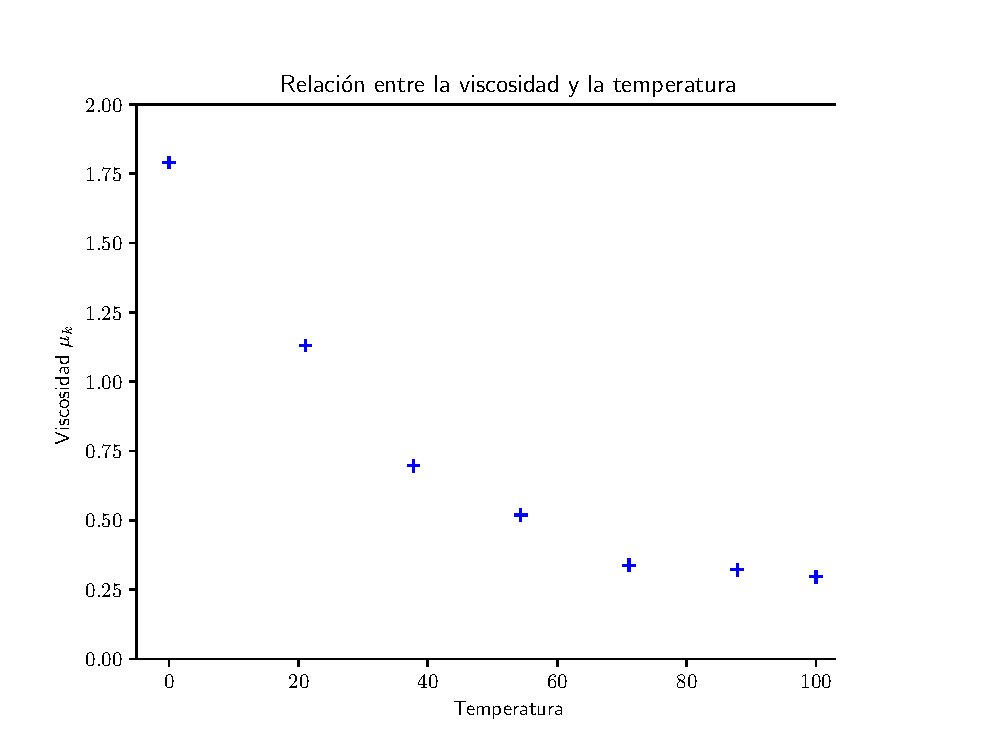
\includegraphics[scale=0.575]{Imagenes/Intro_Interpolacion_01.eps}
\end{figure}
\end{frame}
\begin{frame}
\frametitle{¿Cómo calcular los datos faltantes?}
\begin{figure}
    \centering
    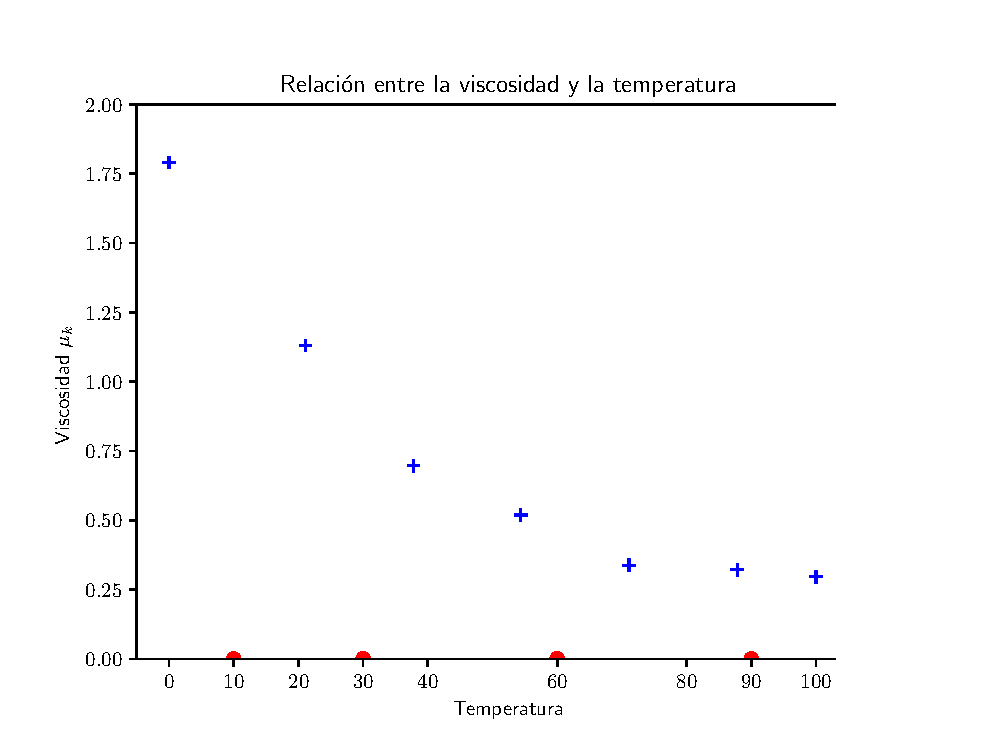
\includegraphics[scale=0.575]{Imagenes/Intro_Interpolacion_02.eps}
\end{figure}
\end{frame}
\begin{frame}
\frametitle{Una interpolación lineal}
\begin{figure}
    \centering
    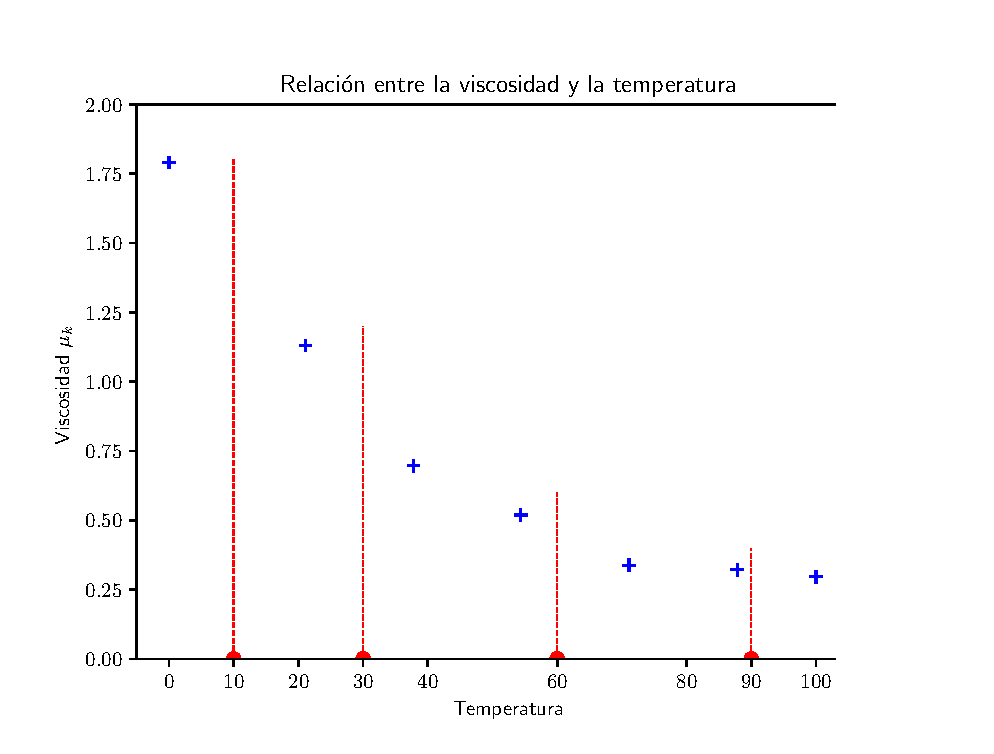
\includegraphics[scale=0.575]{Imagenes/Intro_Interpolacion_03.eps}
\end{figure}
\end{frame}
\begin{frame}
\frametitle{Una interpolación lineal}
\begin{figure}
    \centering
    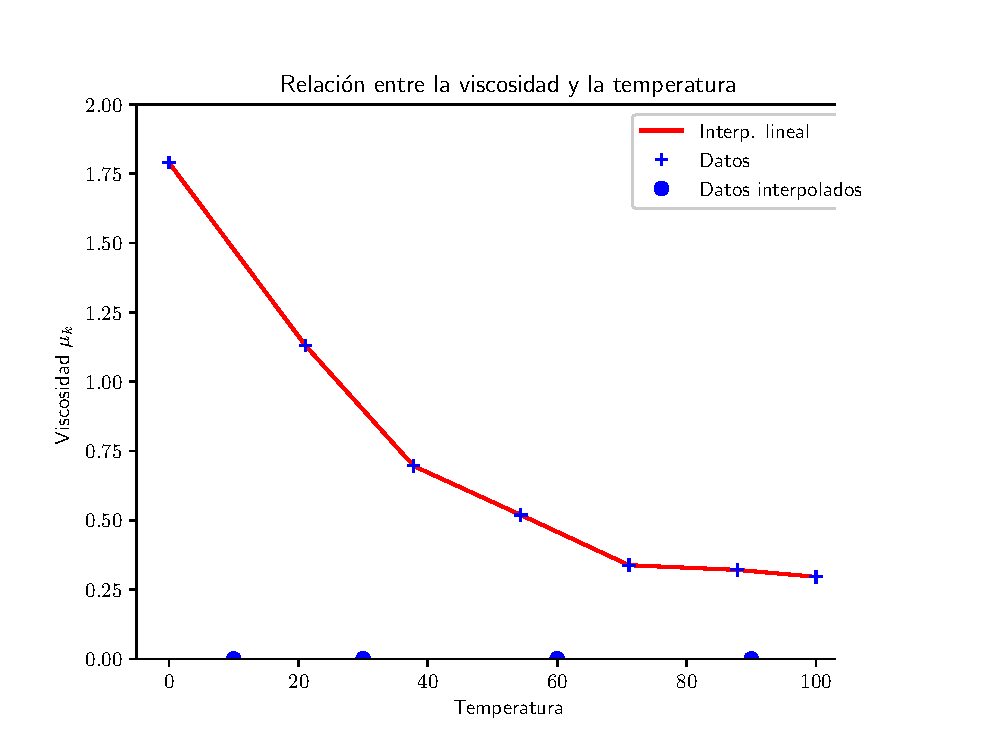
\includegraphics[scale=0.575]{Imagenes/Intro_Interpolacion_04.eps}
\end{figure}
\end{frame}
\begin{frame}
\frametitle{Una interpolación cuadrática}
\begin{figure}
    \centering
    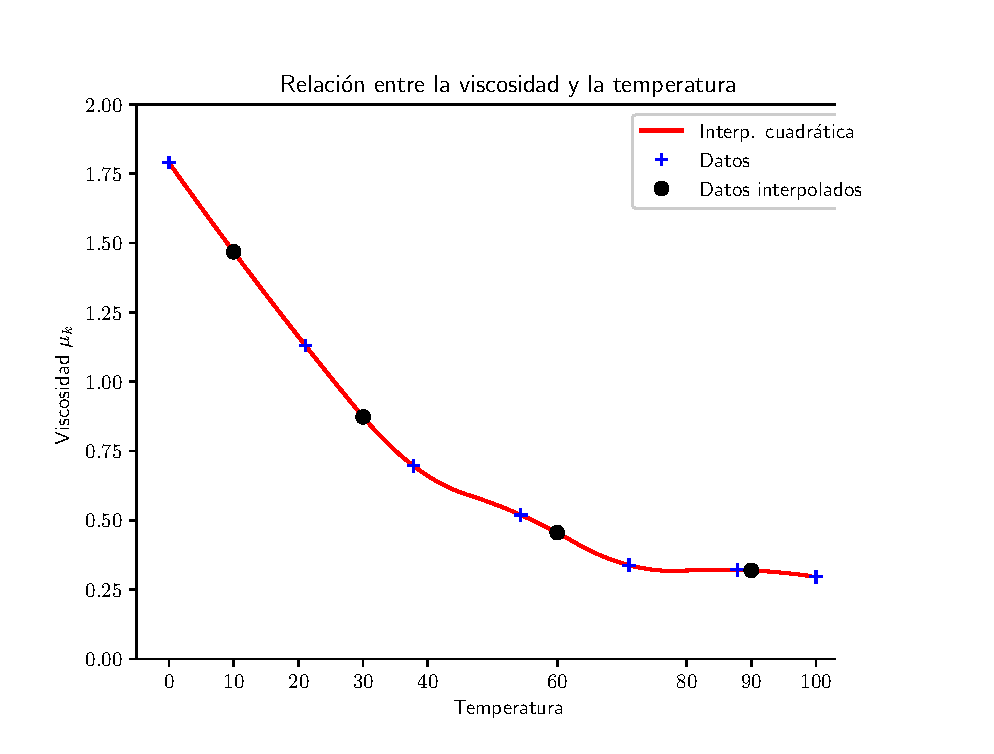
\includegraphics[scale=0.575]{Imagenes/Intro_Interpolacion_05.eps}
\end{figure}
\end{frame} 


\subsection*{Cálculo de raíces}

\begin{frame}
\frametitle{Cálculo de raíces}
\setbeamercolor{item projected}{bg=auburn,fg=aureolin}
\setbeamertemplate{enumerate items}{%
\usebeamercolor[bg]{item projected}%
\raisebox{1.5pt}{\colorbox{bg}{\color{fg}\footnotesize\insertenumlabel}}%
}
\begin{enumerate}[<+->]
\item Bisección.
\item Método de la secante.
\item Falsa posición.
\item Newton - Raphson.
\end{enumerate}
\end{frame}
\begin{frame}
\frametitle{Encontrando raíces de una función}
\begin{figure}
    \centering
    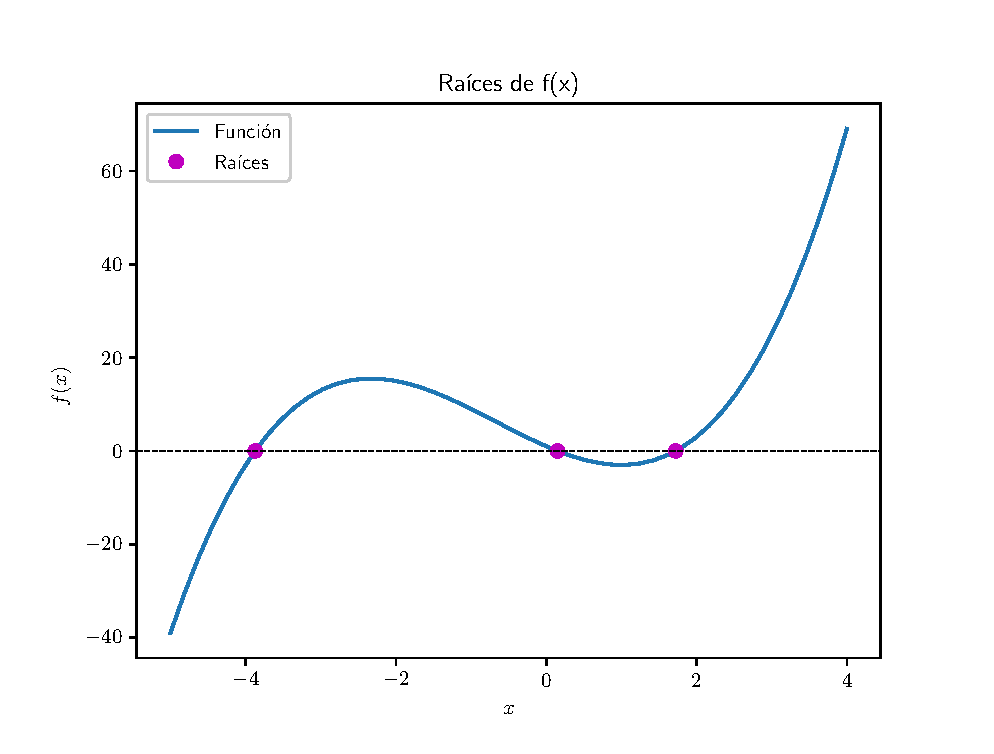
\includegraphics[scale=0.6]{Imagenes/Encuentra_Raices_01.eps}
\end{figure}
\end{frame}

\subsection*{Diferenciación}

\begin{frame}
\frametitle{Diferenciación numérica}
\setbeamercolor{item projected}{bg=babyblue,fg=cadmiumgreen}
Método de diferencias:
\setbeamertemplate{enumerate items}{%
\usebeamercolor[bg]{item projected}%
\raisebox{1.5pt}{\colorbox{bg}{\color{fg}\footnotesize\insertenumlabel}}%
}
\begin{enumerate}[<+->]
\item Hacia adelante.
\item Hacia atrás.
\item Centrales.
\item De orden mayor.
\end{enumerate}
\end{frame}

\subsection*{Integración}

\begin{frame}
\frametitle{Integración numérica}
\setbeamercolor{item projected}{bg=brightgreen,fg=brandeisblue}
\setbeamertemplate{enumerate items}{%
\usebeamercolor[bg]{item projected}%
\raisebox{1.5pt}{\colorbox{bg}{\color{fg}\footnotesize\insertenumlabel}}%
}
\begin{enumerate}[<+->]
\item Fórmulas Newton-Cotes.
\item Fórmulas Gaussianas.
\end{enumerate}
\end{frame}
\begin{frame}
\frametitle{Fórmulas Newton-Cotes}
\setbeamercolor{item projected}{bg=bronze,fg=bubblegum}
\setbeamertemplate{enumerate items}{%
\usebeamercolor[bg]{item projected}%
\raisebox{1.5pt}{\colorbox{bg}{\color{fg}\footnotesize\insertenumlabel}}%
}
\begin{enumerate}[<+->]
\item Trapecio.
\item Trapecio compuesta.
\item Trapecio recursiva.
\item Simpson $1/3$
\item Simpson $3/8$
\item Método de Romberg.
\end{enumerate}
\end{frame}
\begin{frame}
\frametitle{Aproximación polinomial de $f(x)$}
\begin{center}
    \begin{tikzpicture}[font=\footnotesize, scale=1.25]
        \draw [->] (0,0) -- node [near end, left]{$f(x)$} (0,3);
        \draw [->] (0,0) -- (7,0);
        \draw (7.4,0) node {x};
        \draw [blue] (1,0.5) .. controls(2.5,2) .. (6,0.4);
        \foreach \x in {1,1.5,...,6} \draw (\x,0) circle (0.03cm);
        \draw (1,-0.3) node {$x_{0}$};
        \draw (1,-0.7) node {a};
        \draw (1.5,-0.3) node {$x_{1}$};
        \draw (2,-0.3) node {$x_{2}$};
        \draw (2.5,-0.3) node {$x_{3}$};
        \draw (3,-0.3) node {$x_{4}$};
        \draw (5.5,-0.3) node {$x_{n-1}$};
        \draw (6,-0.3) node {$x_{n}$};
        \draw (6,-0.7) node {b};
        \draw [dashed] (1,0) -- (1,0.5);
        \draw [dashed] (1.5,0) -- (1.5,1.05);
        \draw [dashed] (2,0) -- (2,1.37);
        \draw [dashed] (2.5,0) -- (2.5,1.6);
        \draw [dashed] (3,0) -- (3,1.56);
        \draw [dashed] (3.5,0) -- (3.5,1.48);
        \draw [dashed] (4,0) -- (4,1.27);
        \draw [dashed] (4.5,0) -- (4.5,1.09);
        \draw [dashed] (5,0) -- (5,0.85);
        \draw [dashed] (5.5,0) -- (5.5,0.65);
        \draw [dashed] (6,0) -- (6,0.43);
        \draw [<->] (2.5,1) -- node [midway, below] {h} (3,1);
    \end{tikzpicture}
\end{center}
\end{frame}


\begin{frame}
\frametitle{Fórmulas Gaussianas}
\setbeamercolor{item projected}{bg=cadetblue,fg=bubbles}
\setbeamertemplate{enumerate items}{%
\usebeamercolor[bg]{item projected}%
\raisebox{1.5pt}{\colorbox{bg}{\color{fg}\footnotesize\insertenumlabel}}%
}
\begin{enumerate}[<+->]
\item Polinomios ortogonales.
\item Gauss-Chebyshev.
\item Gauss-Hermite.
\item Gauss-Legendre.
\end{enumerate}
\end{frame}

\section{Programas matemáticos}
\frame{\tableofcontents[currentsection, hideothersubsections]}
\subsection{Otro software}

\begin{frame}
\frametitle{¿Es necesario python?}
Si bien es cierto que existen programas o softwares tanto de pago como de tipo GNU, enfocados al cálculo numérico, \pause nos podemos preguntar: ¿por qué hacerlo con \python?
\end{frame}
\begin{frame}
\frametitle{Software matemático}
\begin{figure}
    \centering
    \only<1>{
\includegraphics[scale=0.35]{Imagenes/gnu-octave-logo-lnx.png}}
    \only<2>{
\includegraphics[scale=0.35]{Imagenes/scilab-computer.png}}
    \only<3>{
\includegraphics[scale=0.5]{Imagenes/Wolfram-logo.png}}
    \only<4>{
\includegraphics[scale=0.35]{Imagenes/logo-MATLAB.png}}
    \only<5>{
\includegraphics[scale=0.15]{Imagenes/julia-computing_hd-logo.png}}
    \only<6>{
\includegraphics[scale=0.7]{Imagenes/java-logo.png}}
\end{figure}
\end{frame}
\begin{frame}
\frametitle{Sintaxis en cada programa}
Cada programa/lenguaje requiere conocer su propia sintaxis y con ello, es posible resolver cada uno de los ejercicios que veremos.
\end{frame}
\begin{frame}
\frametitle{Ventaja académica}
La gran ventaja académica que tenemos al revisar la base conceptual de los procedimientos, \pause es que podremos reproducirlos en cualquiera de los lenguajes que tengamos a disposición.
\\
\bigskip
\pause
Mientras que si aprendemos la sintaxis propia, dependeremos exclusivamente de esa herramienta.
\end{frame}

\end{document}